\pagestyle{plain}
\setcounter{page}{1}
\pagenumbering{arabic}
% \thispagestyle{empty}
\section{Introdução}
	O teor de manganês é uma característica química de grande importância para os produtos de aços planos. A incorporação deste elemento ao aço é obtida pela adição de ligas de manganês durante o vazamento do convertedor e/ou nos processos posteriores de metalurgia de panela.
	
	Uma parte do manganês adicionado não é incorporada devido, principalmente, à reação com o oxigênio presente no aço e na escória. O rendimento de incorporação do manganês é uma variável importante para o controle do custo de produção pois o desembolso com ligas de manganês foi de R\$ 593 milhões nos últimos cinco anos representando 2,6\% \cite{r2acu} do custo da placa bruta produzida em 2013.
	
	Neste trabalho, é feita uma análise de dados de processo utilizando as técnicas de Projetos de Experimentos para determinar a constribuição relativa dos seguintes fatores no rendimento de incorporação do manganês adicionado durante o vazamento do convertedor:
	\begin{itemize}\itemsep4pt \parskip0pt \parsep0pt
		\item{nível de oxidação da corrida no final de sopro;}
		\item{passagem de escória no vazamento; e}
		\item{teor de manganês objetivado e}
	\end{itemize}	
	
	O Rendimento calculado apresentou grande variação devido à incerteza introduzida no cálculo pela falta de dados, principalmente do peso de aço na panela de modo que o efeito dos fatores estudados não resotu evidente.
\section{Visão geral da utilização das ligas de manganês}
	O desembolso total por fonte de manganês nos últimos cinco anos é apresentado na Figura (\ref{fig:evol}). Nos últimos cinco anos, o gasto com ligas de manganês totalizou R\$593 milhões. 
	
	A partir do ano 2010, o desembolso total foi reduzido, principalmente, devido à redução de gastos com FeMn baixo fósforo, resultado de uma combinação entre menor consumo especíco e menor custo de aquisição. A redução no consumo específico do FeMn BP deveu-se à substituição deste por FeMn AC na Aciaria 2.

	A utilização do FeMn AC, a liga de manganês de menor custo, era restrita à Aciaria 1 até outubro de 2010 quando houve o \textit{start up} de três novos silos no sistema de ferroligas dos convertedores 4 e 5 cujo objetivo foi o de permitir substituir o FeMn BP pelo FeMn AC nos aços menos exigentes. 
	
	A Figura (\ref{fig:evol_custo}) apresenta a evolução do custo das diferentes ligas de manganês. É observada a redução do custo de aquisição do FeMn BP e do manganês eletrolítico. A tendência de preço do FeMn BP pode, no curto prazo, inviabilizar a utilização do FeMn MC que pode ser substituida pelo FeMn BP com benefício adicional da redução do \textit{input} de fósforo.

	Em julho de 2010 foi alterado o procedimento para refino de aços BH para aproveitar o FeMn MC para incorporação de traços de carbono ao aço para reduzir a recusa por carbono baixo\cite{it20}. Esta mudança resultou no menor consumo de Mn eletrolítico que foi substituído por FeMn MC, com benefícios para a qualidade do aço e redução de custo.
		\begin{figure}[H]
			\centering
			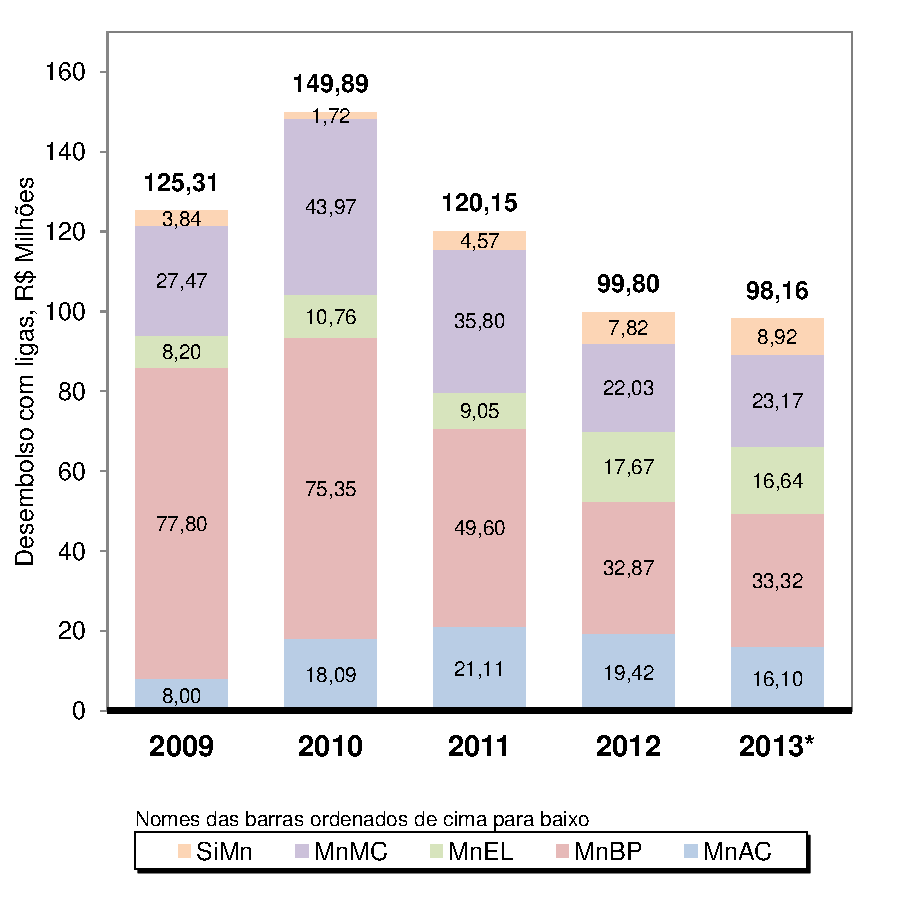
\includegraphics[scale=0.55, bb=0 0 432 432, trim=0in 0in 0in 0in]{figures/fig02-excel.pdf} %left, bottom, right and top
			\caption{Gasto total com ligas de manganês em R\$ milhões. Fonte: sistema R3, transação CKM3.}
			\label{fig:evol}
		\end{figure}		
		\begin{figure}[H]
			\centering
			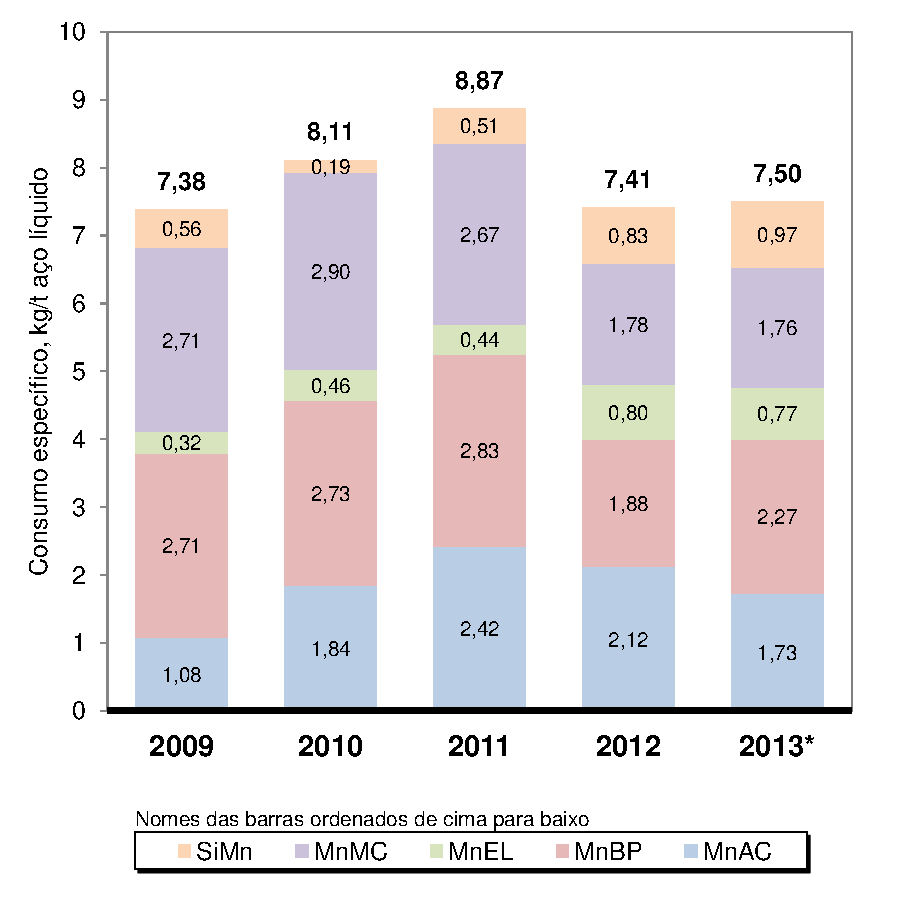
\includegraphics[scale=0.55, bb=0 0 432 432, trim=0in 0in 0in 0in]{figures/fig04-excel.pdf} %left, bottom, right and top
			\caption{Consumo específico das ligas de manganês. Fonte: sistema R3, transação CKM3.}
			\label{fig:evol_kgt}
		\end{figure}		
\section{Metodologia}	
	O principal fenômeno relacionado ao rendimento do manganês adicionado durante o vazamento do convertedor é a oxidação do manganês. Concorre para maior oxidação uma série de fatores como: o nível de oxidação do aço onde a liga será dissolvida; o peso de escória que passa para a panela pois na escória encontram-se óxidos instáveis que são fonte de oxigênio; a adição concomitante com  outras ligas com poder desoxidante e o instante do inicio da descarga da liga em relação ao início do vazamento. Outros fatores aparecem como confundidores pois são obstáculos à correta avaliação do rendimento. Dentre os principais confundidores pode-se citar o teor de manganês real de cada liga e o peso de aço na panela.
	
		\begin{figure}[H]
			\centering
			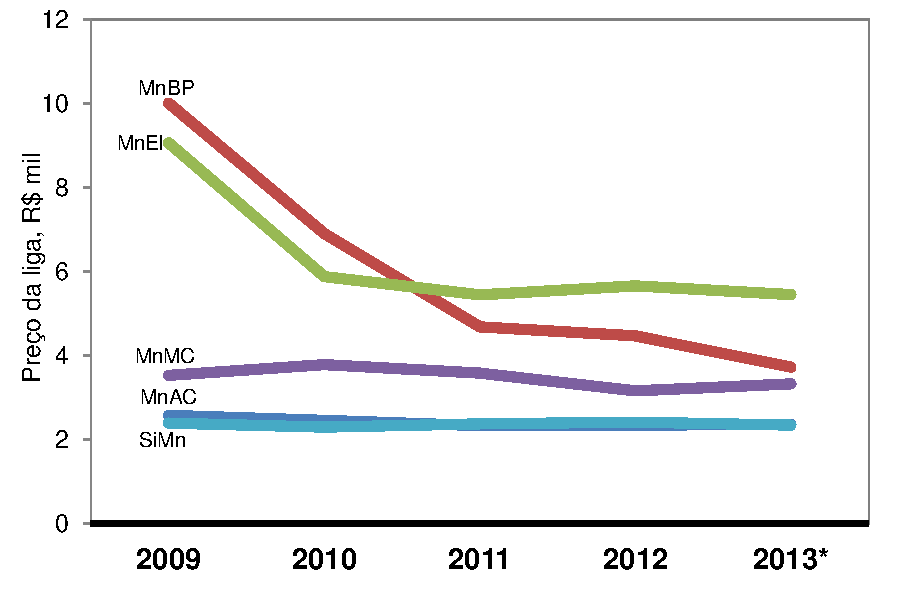
\includegraphics[scale=0.55, bb=0 0 432 288, trim=0in 0in 0in 0in]{figures/fig03-excel.pdf} %left, bottom, right and top
			\caption{Evolução do preço médio do estoque das ligas de manganês.  Fonte: sistema R3, transação CKM3.}
			\label{fig:evol_custo}
		\end{figure}						
	O efeito dos fatores sobre o rendimento do manganês foi estudado utilizando a técnica de Projeto de Experimentos (DOE, do inglês, \textit{Design of Experiments}) utilizando uma planilha eletrônica no Excel. Normalmente, os experimentos são planejados antes de serem conduzidos mas neste trabalho a técnica foi adaptada para utilizar dados de processo.
	
	Foi escolhido um experimento fatorial para estudar o efeito de 3 fatores sobre o rendimento do manganês. A Tabela (\ref{tab:levels}) apresenta um resumo do experimento. Normalmente, os experimentos com três fatores em dois níveis consistem de 8 observações ($2^3$), contudo foi escolhido um fator adicional, o grau de desoxidação do aço (AA/AS), para ser bloqueado. 
	\begin{table}[H]
	\caption{Fatores juntamente com os valores que foram utilizados na definição dos níveis baixo e alto.}
	\label{tab:levels}
	\begin{center}
		\begin{footnotesize}
			\begin{tabular}{lcc}
				\hline
				Fator/Nível & (-1) & (+1) \\
				\hline \hline
				[O], ppm		&	400 a 600	&	1100 a 1500	\\
				Escória			&	0	a 100	&	1000 a 1500	\\
				Visado, pontos  &	50	a  70	&	 100 a  120	\\
				\hline
			\end{tabular}
		\end{footnotesize}	
	\end{center}
	\end{table}
	A oxidação do aço ao final de sopro é medido utilizando um sensor de sub-lança específico. As corridas com medição de teor de oxigênio livre entre 400 e 600 ppm foram escolhidas para representar o nível baixo  deste fator (-1) enquanto que o nível alto (+1) é representado pelas corridas com oxigênio livre entre 1100 e 1500 ppm.
	
	O índice de passagem de escória é determinado pela diferença de emissividade entre o aço e a escória na faixa do infra-vermelho. O sistema responsável por esta medição foi instalado em setembro de 2010 pelo fabricante AMEPA. As corridas com índice de escória entre 1000 e 1500 representam as corridas com passagem de escória e valores inferiores a 100 representam as corridas sem passagem de escória.
	
	Para o teor de manganês visado, os níveis foram selecionados de forma a atender dois requisitos: diferença sensível entre os níveis e representatividade nas corridas pois é preciso que se encontre no banco de dados corridas que combinem os 8 diferentes níveis dos fatores para cada tratamento. Estes critérios foram atendidos para corridas com manganês visado entre 50 e 70 pontos para o nível baixo e entre 100 e 120 pontos para o nível alto.
	
	Neste estudo, foram utilizados dados históricos como variável resposta do experimento projetado. O levantamento de dados resultou numa quantidade heterogênia de corridas distribuidas entre os diferentes tratamentos. Foram utilizadas corridas de 2013 que totalizaram 111 observações. Para adaptar a metodologia, foram aventadas três possibilidades: a seleção aleatória das corridas, a utilização do \textit{bootstapping}\cite{wiki:boot} como forma de reamostragem e a utilização do valor médio do rendimento para cada tratamento. Optou-se pela utilização do rendimento médio do tratamento por ser a alternativa mais simples que não requereria a utilização de nenhuma programação no Excel.
	\subsubsection{Cálculo do rendimento do manganês}
		\label{sec:calcrend}
		O rendimento da adição do manganês foi calculado para as corridas que possuem análise química do aço antes e após o vazamento utilizando a Equação (\ref{eq:rend}):
			\begin{equation}
			\label{eq:rend}
			\eta = \frac{([Mn]_p - [Mn]_b)\times W_{cm} \times \eta_m}{10 \times W_{Mn}},
			\end{equation}
		\noindent onde $[Mn]_p$ e $[Mn]_b$ representam os teores de manganês da amostra de panela e de fim de sopro, em pontos\footnote{1\% em peso de manganês equivale a 100 pontos.}, respectivamente; $W_{cm}$ é o peso total da carga metálica em kg; $\eta_m$ é o rendimento metálico do convertedor, fixado em 91\%, e $W_{Mn}$ é o peso de manganês elementar adicionado calculado como $\sum (w_i x_i)$ em que $w_i$ é o peso da \textit{i-ésima} liga de manganês, em kg e $x_i$ é o teor percentual de manganês da \textit{i-ésima} liga.
		
		A aplicação da Equação (\ref{eq:rend}) apresenta as seguintes desvantagens: o peso de aço na panela não é medido pois não há balança. Mesmo que houvesse haveria ainda a influência do peso de escória e do revestimento da panela para dificultar a determinação do peso de aço. Além disso, a amostra de panela nem sempre é representativa pois a amostragem pode ser feita sem  homogeneização suficiente. Por último, o peso de manganês elementar é calculado com base no teor médio da análise dos ferroligas e, portanto, não é conhecido. 		
		\begin{table}[H]
		\caption{Experimento fatorial completo para o rendimento de manganês adicionado durante o vazamento do convertedor.}
		\label{tab:doe}
			\begin{footnotesize}
			\begin{tabular}[c]{ccccccc}
				\hline
				Trat. & O [ppm] & Escória & Visado & Grau & Rendimento & N \\
				\hline \hline	
				1 & -1 & -1 & -1 & AA & 0,846 & 11   \\
				2 & -1 & -1 & -1 & AS & 0,827 & 15   \\
				3 & -1 & -1 & +1 & AA & 0,884 & 2    \\
				4 & -1 & -1 & +1 & AS & 0,834 & 25   \\
				5 & -1 & +1 & -1 & AA & 0,842 & 8    \\
				6 & -1 & +1 & -1 & AS & 0,831 & 5    \\
				7 & -1 & +1 & +1 & AA & 0,781 & 6    \\
				8 & -1 & +1 & +1 & AS & 0,850 & 9    \\
				9 & +1 & -1 & -1 & AA & 0,998 & 1    \\
				10& +1 & -1 & -1 & AS & 0,826 & 2    \\
				11& +1 & -1 & +1 & AA & 0,886 & 3    \\
				12& +1 & -1 & +1 & AS & 0,946 & 15   \\
				13& +1 & +1 & -1 & AA & 0,794 & 3    \\
				14& +1 & +1 & -1 & AS & 0,801 & 1    \\
				15& +1 & +1 & +1 & AA & 0,808 & 3    \\
				16& +1 & +1 & +1 & AS & 0,987 & 2    \\
				\hline
			\end{tabular}
			\end{footnotesize}
		\end{table}		
\section{Resultados}
		O rendimento obtido do banco de dados para cada tratamento é apresentado na Tabela (\ref{tab:doe}). Com estes dados é construído o gráfico com os efeitos principais, mostrado na Figura (\ref{fig:main}). Para determinação do efeito de cada fator, o rendimento médio é calculado no nível alto e baixo do fator estudado, independentemente do nível dos demais fatores. 
		
		A análise da Figura (\ref{fig:main}) mostra que as corridas com maior teor de oxigênio fim de sopro apresentaram rendimento superior. A explicação pode estar relacionada a outras variáveis acopladas ao teor de oxigênio, como a temperatura fim de sopro. A partição do manganês entre o aço e a escória é influenciada pela temperatura do banho e como a reação de oxidação é exotérmica, a aplicação do princípio de \textit{Le Châtelier} leva à conclusão de que temperaturas mais elevadas são favoráveis à obtenção de maiores teores de manganês no metal líquido\cite{barao}.

		O efeito da passagem de escória mostrou-se deletério. As corridas com maior peso de escória apresentaram rendimento menor. Sendo a escória uma grande fonte de oxigênio este resultado concorda com o esperado.
		
		Por último, o rendimento foi diretamente proporcional ao teor de manganês visado. Se considerarmos um peso fixo de manganês a ser oxidado, essa parcela será menos significativa quanto maior for a adição. Portanto, nas corridas com maior adição existe a \textit{tendência} de maior rendimento percentual.
		
		O estudo para determinar a significância dos fatores e suas interações foi conduzido utilizando a Análise de Variância (ANOVA)\cite{wiki:anova} numa planilha do Excel.
		
		Para aplicação da Análise de Variança é preciso construir um modelo linear com os dados da Tabela (\ref{tab:doe}). O primeiro passo é determinar os níveis das interações. As interações e os respectivos níveis são apresentados na Tabela (\ref{tab:inter}).		
		\begin{table}[H]
		\caption{Níveis determinados para as interações dos fatores. A: [O] ppm, B: Escória e C: Mn visado.}
		\label{tab:inter}
			\begin{center}
			\begin{footnotesize}
				\begin{tabular}[c]{cccc|cccc}
				\hline
				Trat. & A & B & C & A*B & A*C & B*C & A*B*C \\
				\hline \hline
				1&-1&-1&-1&+1&+1&+1&-1	\\
				2&-1&-1&+1&+1&-1&+1&+1	\\
				3&-1&+1&-1&-1&+1&-1&+1	\\
				4&-1&+1&+1&-1&-1&-1&-1	\\
				5&+1&-1&-1&-1&-1&-1&+1	\\
				6&+1&-1&+1&-1&+1&-1&-1	\\
				7&+1&+1&-1&+1&-1&+1&-1	\\
				8&+1&+1&+1&+1&+1&+1&+1	\\
				\hline
				\end{tabular}
			\end{footnotesize}
			\end{center}
		\end{table}
		O modelo linear tem a forma geral:
		\begin{equation}
		\begin{split}
		\label{eq:modelo}
			\hat{\eta} &= \bar{\eta} + \alpha_a A + \alpha_b B + \alpha_c C + \\ & + \alpha_{ab} AB + \alpha_{ac} AC + \alpha_{bc} BC + \\ & +  \alpha_{abc} ABC +\epsilon,
		\end{split}
		\end{equation}
		\noindent onde, $\hat{\eta}$ é o rendimento estimado pelo modelo linear; $\bar{\eta}$ é o rendimento médio obtido em todos os tratamentos, $\epsilon$ é o efeito aleatório de tudo que não foi modelado tal que $\epsilon \sim N(0, \sigma^2)$ e os coeficientes $\alpha_a$ até $\alpha_{abc}$ são calculados pela Equação (\ref{eq:fat}):
		\begin{equation}
		\label{eq:fat}
			\alpha_i = \frac{\hat{\eta}_i^{(+1)} - \hat{\eta}_i^{(-1)} }{2},
		\end{equation}
		\begin{figure}[H]
			\centering
			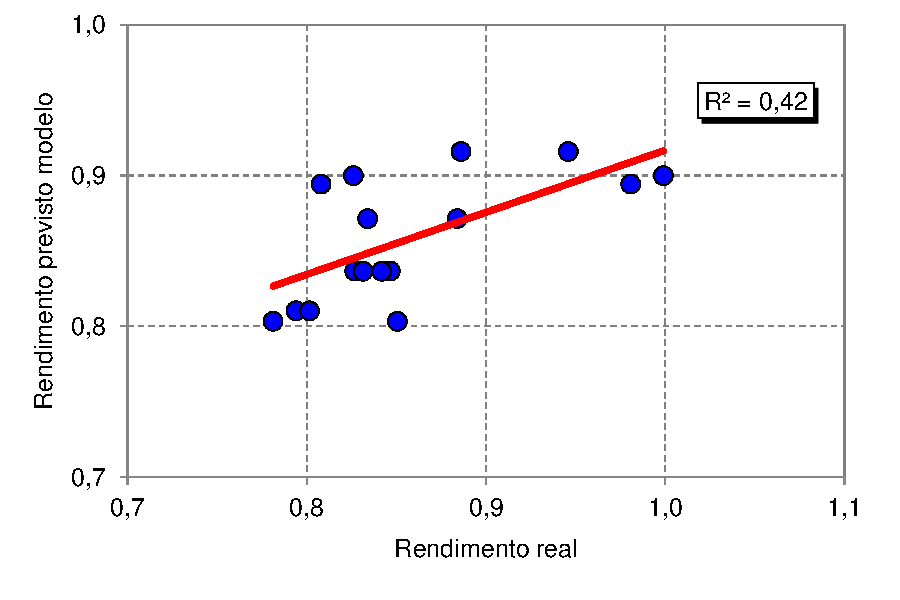
\includegraphics[scale=0.55, bb=0 0 432 288, trim=0in 0in 0in 0in]{figures/fig06-excel.pdf} %left, bottom, right and top
			\caption{Rendimento real e previsto pelo modelo.}
			\label{fig:reg}
		\end{figure}
		\noindent onde $\hat{\eta}_i^{(+1)}$ é o valor médio do rendimento avaliado apenas para o nível alto do \textit{i-ésimo} fator ou interação e $\hat{\eta}_i^{(-1)}$ é o análogo do anterior para o nível baixo do \textit{i-ésimo} fator ou interação.
		
		A Figura (\ref{fig:reg}) apresenta a relação entre o rendimento previsto pelo modelo formulado na Equação (\ref{eq:modelo}) com os parâmetros obtidos com a aplicação da Equação (\ref{eq:fat}) sob os dados da Tabela(\ref{tab:doe}). Os parâmetros utilizados são apresentados na Tabela (\ref{tab:coef}).
		
		O valor médio dos resíduos foi igual a zero e o teste de normalidade de Anderson-Darling\cite{wiki:ad} foi conduzido para testar a hipótese de normalidade. A estatística do teste AD foi 0,3845 que corresponde a um p-valor de 0,3512 que não permite rejeitar a hipótese de que os resíduos são normalmente distribuídos.		
		\begin{table}[H]
			\caption{Coeficientes do modelo linear para o rendimento da adição de manganês. A: [O] ppm, B: Escória e C: Mn visado.}
			\label{tab:coef}
				\begin{center}
				\begin{footnotesize}
					\begin{tabular}{cccc}
						\hline
							Termo 		& Coef.   & SE Coef. & T \\
						\hline \hline
							Intercepto 	&  0,8585 & 0,0126 &  68,0974 \\
							A 			&  0,0216 & 0,0126 &  1,71061 \\
							B 			& -0,0224 & 0,0126 & -1,77963 \\
							C 			&  0,0127 & 0,0126 &  1,00739 \\
							A*B 		& -0,0116 & 0,0126 & -0,92326 \\
							A*C 		&  0,0123 & 0,0126 &  0,97603 \\
							B*C 		&  0,0063 & 0,0126 &  0,49699 \\
							A*B*C 		&  0,0170 & 0,0126 &  1,34955 \\						
						\hline
					\end{tabular}
				\end{footnotesize}
				\end{center}			
		\end{table}
		Na Tabela (\ref{tab:coef}), além dos valores estimados para os coeficientes do modelo linear, são apresentados os valores do Erro Padrão (SE, \textit{Standard Error}) e da estatística-T calculada com o Erro Padrão. O Erro Padrão, $S_e$,é utilizado para testar a significância do coeficiente. Um coeficiente é considerado significativo se o intervalo de confiança construído ao nível de significância, $\alpha$, com o erro padrão não contiver o zero. Caso o valor nulo esteja contido no intervalo de confiança então não há evidência para rejeitar a hipótese de que o coeficiente tem valor zero. Coeficientes com valor nulo não são relevantes como variáveis explicativas de fenômenos modelados com modelos lineares.
		
		O Erro Padrão foi determinado com base na raiz quadrada do erro quadrático médio, o RMSE (\textit{Root Mean Squared Error}) com graus de liberdade igual a $(n-2)$, onde $n$ é o número de observações, conforme Equação (\ref{eq:mse}).
		\begin{equation}
		\label{eq:mse}
		S_e = \sqrt{\frac{1}{(n-2)}  \sum_{i=0}^n \left( \eta_i - \hat{\eta_i} \right)^2},
		\end{equation}
		\noindent onde $\eta_i$ é o rendimento do \textit{i-ésimo} experimento; $\hat{\eta_i}$ é o rendimento previsto pelo modelo para o \textit{i-ésimo} experimento e $n$ é o número de observações.
		
		A estatística-T é obtida pela divisão do valor estimado para coeficiente pelo Erro Padrão é também chamada de Efeito Padronizado. O efeito de um fator ou interação é considerado significativo se o seu Efeito Padronizado for superior a um valor limiar. O valor limiar de significância foi calculado o nível de 5\% usando a distribuição \textit{t de Student} com 8 graus de liberdade. No Excel, o valor inverso da distribuição \textit{t} com 8 graus de liberdade pode ser obtido com a  fórmula {\small \texttt{=INVT(5\%;8)}} que retorna o valor de 2,306. 
		\begin{figure}[H]
			\centering
			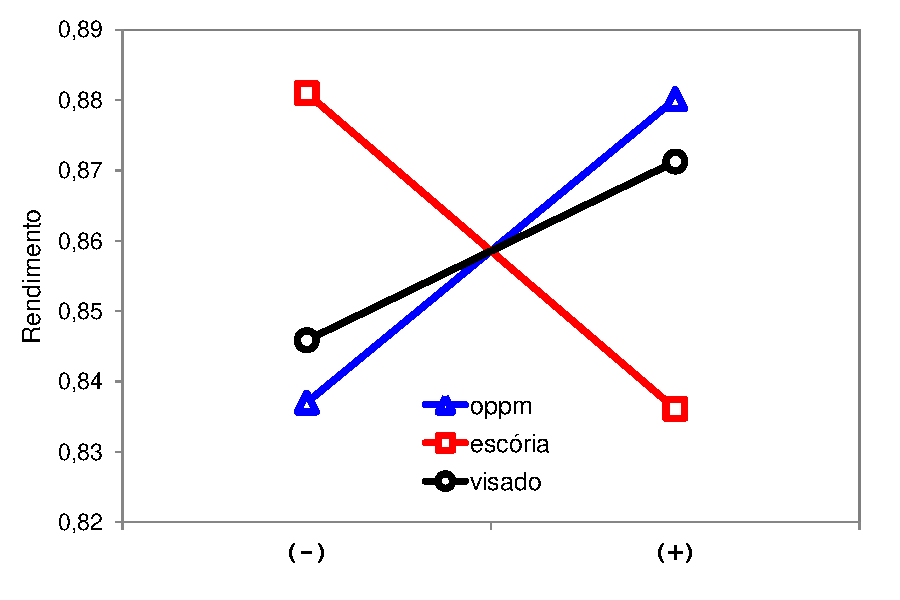
\includegraphics[scale=0.55, bb=0 0 432 288, trim=0in 0in 0in 0in]{figures/fig05-excel.pdf} %left, bottom, right and top
			\caption{Efeitos principais sobre o rendimento da adição de manganês no vazamento.}
			\label{fig:main}
		\end{figure}		
		O gráfico de Paretto com o efeito padronizado dos fatores e interações mostra que nenhum fator ou interação exerceu efeito significativo sobre o rendimento da adição. 
		\begin{figure}[H]
			\centering
			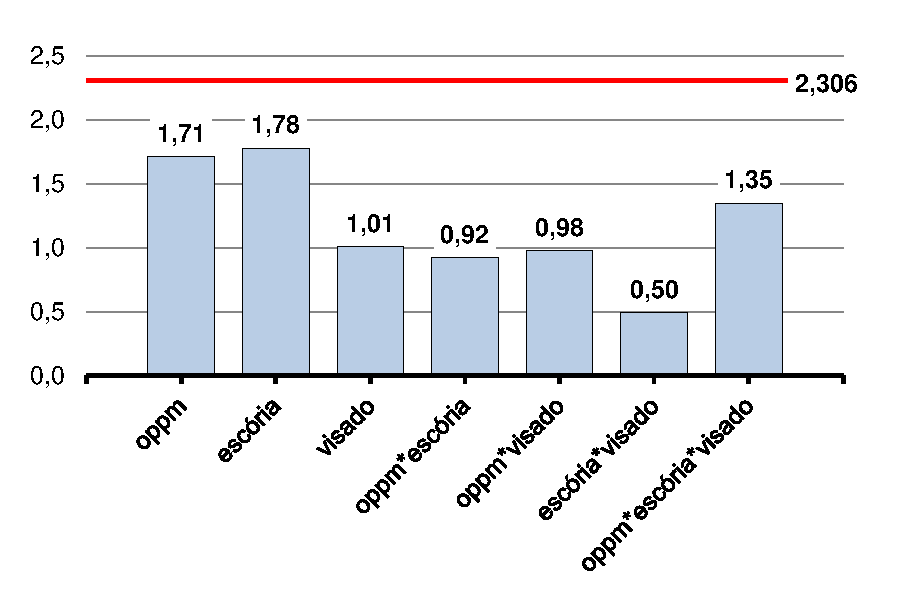
\includegraphics[scale=0.55, bb=0 0 432 288, trim=0in 0in 0in 0in]{figures/fig07-excel.pdf} %left, bottom, right and top
			\caption{Efeito padronizado dos fatores e interações. Ao nível de significância de 5\% a estatística-T limiar é 2,306.}
			\label{fig:pareto}
		\end{figure}		
		O rendimento é melhor explicado pela média global do que pelo efeito de qualquer dos fatores. Este resultado não significa que os fatores estudados não são relevantes. Significa que o rendimento não pode ser calculado com precisão suficiente para detectar a fiderença entre os tratamentos.
\section{Conclusões}
		Foram utilizados dados históricos para compor os tratamentos de um Projeto de Experimento fatorial completo para investigar o efeito da oxidação do aço, da passagem de escória e do manganês visado sobre o rendimento das ligas de manganês usadas no vazamento do convertedor. O rendimento foi calculado com o peso de aço estimado por um rendimento metálico fixo de 91\%.
		
		Nenhum dos fatores apresentou efeito significativo sobre o rendimento. A conclusão foi que as estimativas usadas para calcular o rendimento introduziram mais incerteza do que o efeito das variáveis estudadas.
		
		Para permitir a melhoria sobre o rendimento das adições de manganês torna-se necessário desenvolver uma metodologia mais precisa para sua determinação.
